
\section{Traducció a circuits}

En aquesta secció, es descriuen les regles dissenyades per traduir de forma 
automàtica el codi del nostre llenguatge a circuits lògics (expressats en el 
llenguatge \texttt{Verilog}). Les idees fonamentals estan basades en 
l'exposició de \cite{wirth1998hardware} (tot i que s'han ampliat per permetre 
construccions diferents de les mostrades en l'article citat).

Les explicacions d'aquesta secció es basen en diversos diagrames de circuits 
que en faciliten la comprensió. En aquests, s'ha seguit la convenció 
d'utilitzar línies fines per als cables d'un únic bit i línies més gruixudes 
per representar els busos de \(n\) bits (on \(n\) és un nombre especificat per 
l'usuari del llenguatge al principi del programa a traduir; en els subsegüents
diagrames s'utilitzarà \(n=2\) per simplicitat). A més, aquests circuits 
corresponen a l'execució d'un codi i, per tant, s'ha intentat que es 
puguin interpretar d'aquesta manera veient-los ``d'esquerra a dreta'' (en 
particular, quan apareixen diversos senyals amb el mateix nom, el senyal de 
l'esquerra correspon a l'entrada d'aquell fragment de circuit, mentre que el 
senyal de la dreta correspon a la sortida).

Els circuits s'expressen utilitzant només portes lògiques i biestables de 
dos tipus. Els del primer tipus tenen un senyal d'entrada \textsc{d}, un de 
sortida \textsc{q} i un de reinici \textsc{r}. Quan hi ha un flanc ascendent 
del rellotge es canvia el valor de \textsc{q}: si el valor de \textsc{r} és 1, 
aleshores \textsc{q} passa a valdre 0; altrament, el valor de \textsc{q} 
passa a ser el valor de \textsc{d}. Els biestables del segon tipus 
funcionen de forma similar però, a més, tenen un senyal d'activació 
\textsc{e}. Així, quan hi ha un flanc ascendent de rellotge i el valor de 
\textsc{r} és 0, només es canvia el valor de \textsc{q} pel de \textsc{d} si 
el valor de \textsc{e} és 1 (altrament, el valor de \textsc{q} roman 
inalterat). 

Per traduir un programa a \textit{hardware}, es van generant recursivament 
fragments d'un circuit lògic seguint l'estructura de l'AST que representa les 
instruccions del programa. Aquests circuits es componen de dues parts: d'una 
banda, hi ha una part principal del circuit que efectua els càlculs expressats 
en les instruccions del programa; de l'altra, hi ha una segona part igual 
d'important que controla el flux de l'execució (és a dir, activa i desactiva 
els diferents components del primer circuit per garantir que les operacions 
s'efectuen seguint l'ordre correcte). Vegem ara com es tradueixen els 
diferents tipus d'instruccions.

\begin{figure}[ht]
    \centering
    \documentclass[tikz,12pt,border=12pt]{standalone}

\usepackage{mathpazo}
\usepackage[scaled=1.03,varqu]{zi4}
\usepackage[T1]{fontenc}
\usepackage[utf8]{inputenc}
\usepackage{mathtools}
\usepackage{pgf,tikz}
\usetikzlibrary{circuits.logic.US}


\begin{document}

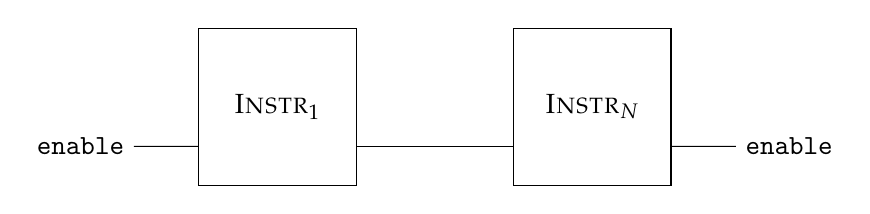
\begin{tikzpicture}[circuit logic US,%
        dot/.style    = {anchor=base,fill,circle,inner sep=1.3pt}]

\node[draw,rectangle,minimum width=2cm,minimum height=2cm] at (1,1) (i1) {$\textsc{Instr}_1$};
\node[draw,rectangle,minimum width=2cm,minimum height=2cm] at (5,1) (in) {$\textsc{Instr}_N$};
\node at (-1.5,0.5) (e_in) {\texttt{enable}};
\node at (7.5,0.5) (e_out) {\texttt{enable}};

\draw ($ (i1.east) + (0,-0.5) $) -- ($ (in.west) + (0,-0.5) $);
\draw (e_in.east) -- ($ (i1.west) + (0,-0.5) $);
\draw ($ (in.east) + (0,-0.5) $) -- (e_out.west);

\end{tikzpicture}

\end{document}




    \caption{Circuit corresponent a una llista de \(N\) instruccions (en el 
        diagrama, per simplicitat, \(N=2\)) consecutives.}
    \label{fig:instr-list}
\end{figure}

Per traduir un bloc d'instruccions consecutives, senzillament cal traduir 
cadascuna de les instruccions per separat i encadenar els senyals d'activació. 
D'aquesta manera, es fa que el senyal de sortida del circuit corresponent a la 
primera instrucció sigui el senyal d'entrada del circuit corresponent a la 
segona instrucció, i així successivament fins a l'última. La 
\autoref{fig:instr-list} mostra la forma dels circuits obtinguts d'aquesta 
forma.

\begin{figure}[ht]
    \centering
    \input{circuits/ifelse}
    \caption{Circuit corresponent a una sentència condicional.}
    \label{fig:if-else}
\end{figure}

La \autoref{fig:if-else} mostra el circuit generat per a una sentència 
condicional. En qualsevol dels casos, primerament cal avaluar la condició i, 
per tant, es genera recursivament el circuit \textsc{Cond} corresponent i s'hi 
col·loca el senyal d'activació de la sentència condicional directament. Com 
que el llenguatge dissenyat treballa amb vectors de \(n\) bits fins i tot per 
a les condicions, cal utilitzar una porta \textit{or} amb entrades cadascun 
d'aquests \(n\) bits per comprovar si la condició es verifica o no (en aquest 
llenguatge, l'únic valor amb el valor lògic fals és el 0). Els dos circuits 
corresponents a les branques condicional i alternativa d'aquesta instrucció, 
\textsc{IfT} i \textsc{IfF}, també es generen recursivament i cal muntar 
un circuit d'activació que n'activi exactament un dels dos (en funció del 
valor de la condició avaluada). A més, aquests circuits s'han d'activar 
justament després que el circuit d'avaluació de la condició. Així, doncs, el 
senyal d'activació del circuit \textsc{IfT} es connecta amb el resultat d'una 
porta \textit{and} amb entrades la condició avaluada i el senyal d'activació 
de sortida de \textsc{Cond}; anàlogament, el senyal d'activació del circuit 
\textsc{IfF} es connecta amb el resultat d'una porta \textit{and} amb entrades 
la condició avaluada negada i el senyal d'activació del circuit de sortida de 
\textsc{Cond}. Finalment, el senyal d'activació resultant després d'aquesta 
instrucció s'ha d'obtenir mitjançant una porta \textit{or} amb els senyals 
d'activació que surten de \textsc{IfT} i \textsc{IfF} (o sigui, la instrucció 
s'acaba d'executar quan alguna de les dues branques condicionals finalitza la 
seva execució). En cas que no hi hagi una branca alternativa (és a dir, un 
\textit{else}), el circuit \textsc{IfF} desapareix i la resta del circuit 
queda exactament igual.

\begin{figure}[ht]
    \centering
    \documentclass[tikz,12pt,border=12pt]{standalone}

\usepackage{mathpazo}
\usepackage[scaled=1.03,varqu]{zi4}
\usepackage[T1]{fontenc}
\usepackage[utf8]{inputenc}
\usepackage{mathtools}
\usepackage{pgf,tikz}
\usetikzlibrary{circuits.logic.US}


\begin{document}

\begin{tikzpicture}[circuit logic US,%
        dot/.style    = {anchor=base,fill,circle,inner sep=1.3pt}]

\node[draw,rectangle,minimum width=2cm,minimum height=2cm] at (0,1.5) (Cond) {\textsc{Cond}};
\node[dot] at (1.5,2) (aux1_cond) {};
\node[or gate,inputs=nn] at (2.5,2) (or_cond) {};
\node[dot] at (3.5,2) (aux2_cond) {};
\node[dot] at (4,1) (aux3_cond) {};
\node[and gate,inputs=nn] at (5,3) (and_enb_if) {};
\node[and gate,inputs=in] at (5,1.1) (and_enb_else) {};
\node[draw,rectangle,minimum width=2cm,minimum height=2cm] at (7,3.5) (WhileT) {\textsc{WhileT}};
\node at (-4.5,1.1) (e_in) {\texttt{enable}};
\node[or gate,inputs=nn] at (-2,1) (or_cond_in) {};
\node at (7,1.1) (e_out) {\texttt{enable}}; 

\draw[very thick] ($ (Cond.east) + (0,0.5) $) -- (aux1_cond);
\draw (aux1_cond) |- (or_cond.input 1);
\draw (aux1_cond) |- (or_cond.input 2);
\draw (or_cond.output) |- (aux2_cond) |- (and_enb_if.input 1); \draw (aux2_cond) |- (and_enb_else.input 1);
\draw ($ (Cond.east) + (0,-0.5) $) -- (aux3_cond);
\draw (and_enb_if.output) |- ($ (WhileT.west) + (0,-0.5) $);
\draw ($ (WhileT.east) + (0,-0.5) $) -- ++(0.5,0) -- ++(0,-3) -- ++(-11.5,0) |- (or_cond_in.input 2);
\draw (aux3_cond) -- (and_enb_else.input 2); \draw (aux3_cond) |- (and_enb_if.input 2);
\draw (e_in) -- (or_cond_in.input 1);
\draw (or_cond_in.output) -- ($ (Cond.west) + (0,-0.5) $); 
\draw (and_enb_else.output) -- (e_out);

\end{tikzpicture}

\end{document}




    \caption{Circuit corresponent a una sentència repetitiva.}
    \label{fig:while}
\end{figure}

El circuit generat per a una sentència repetitiva s'il·lustra a la 
\autoref{fig:while}. El fragment \textsc{Cond} d'aquest (que correspon a 
l'avaluació de la condició) i l'activació de \textsc{WhileT} (corresponent al 
bloc d'instruccions que conforma el cos de la sentència repetitiva) en funció 
del resultat de la condició és igual que el d'una sentència condicional
(sense \textit{else}) i, per tant, n'ometem una descripció en detall. En 
aquest cas, però, el senyal d'activació per al circuit \textsc{Cond} es 
calcula de forma diferent, ja que s'ha de poder repetir després de cada 
iteració. D'una banda, aquest s'ha d'activar quan s'inicia l'execució de la 
instrucció (abans de començar cap iteració); d'altra banda, també cal activar 
l'execució de la condició just després d'executar una iteració del cos de la 
sentència repetitiva. Per tant, es col·loca una porta \textit{or} que té per 
entrades el senyal d'activació d'entrada de la instrucció i el senyal de 
sortida del circuit \textsc{WhileT} i es connecta la sortida d'aquesta porta 
al senyal d'activació d'entrada del circuit \textsc{Cond}.  

Fins al moment ja s'ha explicat el mètode seguit per a la generació dels 
circuits que controlen el flux d'execució del programa. Així, doncs, queda 
descriure els circuits que es generen per a definir les variables i les 
funcions del programa (en aquest document no s'explica com dissenyar un 
circuit per a executar les operacions aritmètiques i lògiques bàsiques, ja 
que no és l'objectiu del projecte; de fet, aquesta tasca es deixa a l'eina de 
síntesi o de simulació del circuit perquè les operacions s'expressen 
directament en la sintaxi de \texttt{Verilog}).

\begin{figure}[ht]
    \centering
    \documentclass[tikz,12pt,border=12pt]{standalone}

\usepackage{mathpazo}
\usepackage[scaled=1.03,varqu]{zi4}
\usepackage[T1]{fontenc}
\usepackage[utf8]{inputenc}
\usepackage{mathtools}
\usepackage{pgf,tikz}
\usetikzlibrary{circuits.logic.US}


%%%%%%%%%%%%%%%%%%%%%%%%%%%%%%%%%%%%%%%%%%%%%%%%%%%%%%%%%%%%%%%%%%%%%%%%%%%%%%%

\makeatletter

% Data Flip Flip (DFF) shape
\pgfdeclareshape{dff}{
  % The 'minimum width' and 'minimum height' keys, not the content, determine
  % the size
  \savedanchor\northeast{%
    \pgfmathsetlength\pgf@x{\pgfshapeminwidth}%
    \pgfmathsetlength\pgf@y{\pgfshapeminheight}%
    \pgf@x=0.5\pgf@x
    \pgf@y=0.5\pgf@y
  }
  % This is redundant, but makes some things easier:
  \savedanchor\southwest{%
    \pgfmathsetlength\pgf@x{\pgfshapeminwidth}%
    \pgfmathsetlength\pgf@y{\pgfshapeminheight}%
    \pgf@x=-0.5\pgf@x
    \pgf@y=-0.5\pgf@y
  }
  % Inherit from rectangle
  \inheritanchorborder[from=rectangle]

  % Define same anchor a normal rectangle has
  \anchor{center}{\pgfpointorigin}
  \anchor{north}{\northeast \pgf@x=0pt}
  \anchor{east}{\northeast \pgf@y=0pt}
  \anchor{south}{\southwest \pgf@x=0pt}
  \anchor{west}{\southwest \pgf@y=0pt}
  \anchor{north east}{\northeast}
  \anchor{north west}{\northeast \pgf@x=-\pgf@x}
  \anchor{south west}{\southwest}
  \anchor{south east}{\southwest \pgf@x=-\pgf@x}
  \anchor{text}{
    \pgfpointorigin
    \advance\pgf@x by -.5\wd\pgfnodeparttextbox%
    \advance\pgf@y by -.5\ht\pgfnodeparttextbox%
    \advance\pgf@y by +.5\dp\pgfnodeparttextbox%
  }

  % Define anchors for signal ports
  \anchor{D}{
    \pgf@process{\northeast}%
    \pgf@x=-1\pgf@x%
    \pgf@y=.5\pgf@y%
  }
  \anchor{CLK}{
    \pgf@process{\northeast}%
    \pgf@x=-1\pgf@x%
    \pgf@y=-.66666\pgf@y%
  }
  \anchor{Q}{
    \pgf@process{\northeast}%
    \pgf@y=0pt%
  }
  \anchor{R}{
    \pgf@process{\northeast}%
    \pgf@x=0pt%
  }
  \anchor{E}{
    \pgf@process{\northeast}%
    \pgf@x=0pt%
    \pgf@y=-\pgf@y%
  }
  % Draw the rectangle box and the port labels
  \backgroundpath{
    % Rectangle box
    \pgfpathrectanglecorners{\southwest}{\northeast}
    % Angle (>) for clock input
    \pgf@anchor@dff@CLK
    \pgf@xa=\pgf@x \pgf@ya=\pgf@y
    \pgf@xb=\pgf@x \pgf@yb=\pgf@y
    \pgf@xc=\pgf@x \pgf@yc=\pgf@y
    \pgfmathsetlength\pgf@x{1.6ex} % size depends on font size
    \advance\pgf@ya by \pgf@x
    \advance\pgf@xb by \pgf@x
    \advance\pgf@yc by -\pgf@x
    \pgfpathmoveto{\pgfpoint{\pgf@xa}{\pgf@ya}}
    \pgfpathlineto{\pgfpoint{\pgf@xb}{\pgf@yb}}
    \pgfpathlineto{\pgfpoint{\pgf@xc}{\pgf@yc}}
    \pgfclosepath

    % Draw port labels
    \begingroup
    \tikzset{flip flop/port labels} % Use font from this style
    \tikz@textfont

    \pgf@anchor@dff@D
    \pgftext[left,base,at={\pgfpoint{\pgf@x}{\pgf@y}},x=\pgfshapeinnerxsep]{\raisebox{-0.75ex}{D}}

    \pgf@anchor@dff@Q
    \pgftext[right,base,at={\pgfpoint{\pgf@x}{\pgf@y}},x=-\pgfshapeinnerxsep]{\raisebox{-.75ex}{Q}}

    \pgf@anchor@dff@R
    \pgftext[top,at={\pgfpoint{\pgf@x}{\pgf@y}},y=-\pgfshapeinnerysep]{R}

    \pgf@anchor@dff@E
    \pgftext[bottom,at={\pgfpoint{\pgf@x}{\pgf@y}},y=\pgfshapeinnerysep]{E}
    \endgroup
  }
}

% Key to add font macros to the current font
\tikzset{add font/.code={\expandafter\def\expandafter\tikz@textfont\expandafter{\tikz@textfont#1}}} 

% Define default style for this node
\tikzset{flip flop/port labels/.style={font=\rmfamily\scriptsize}}
\tikzset{every dff node/.style={draw,minimum width=2cm,minimum 
height=2.828427125cm,inner sep=1mm,outer sep=0pt,cap=round,add 
font=\rmfamily}}

\makeatother

%%%%%%%%%%%%%%%%%%%%%%%%%%%%%%%%%%%%%%%%%%%%%%%%%%%%%%%%%%%%%%%%%%%%%%%%%%%%%%%
%%%%%%%%%%%%%%%%%%%%%%%%%%%%%%%%%%%%%%%%%%%%%%%%%%%%%%%%%%%%%%%%%%%%%%%%%%%%%%%

\makeatletter

% Data Flip Flip (DFF) shape
\pgfdeclareshape{dffne}{
  % The 'minimum width' and 'minimum height' keys, not the content, determine
  % the size
  \savedanchor\northeast{%
    \pgfmathsetlength\pgf@x{\pgfshapeminwidth}%
    \pgfmathsetlength\pgf@y{\pgfshapeminheight}%
    \pgf@x=0.5\pgf@x
    \pgf@y=0.5\pgf@y
  }
  % This is redundant, but makes some things easier:
  \savedanchor\southwest{%
    \pgfmathsetlength\pgf@x{\pgfshapeminwidth}%
    \pgfmathsetlength\pgf@y{\pgfshapeminheight}%
    \pgf@x=-0.5\pgf@x
    \pgf@y=-0.5\pgf@y
  }
  % Inherit from rectangle
  \inheritanchorborder[from=rectangle]

  % Define same anchor a normal rectangle has
  \anchor{center}{\pgfpointorigin}
  \anchor{north}{\northeast \pgf@x=0pt}
  \anchor{east}{\northeast \pgf@y=0pt}
  \anchor{south}{\southwest \pgf@x=0pt}
  \anchor{west}{\southwest \pgf@y=0pt}
  \anchor{north east}{\northeast}
  \anchor{north west}{\northeast \pgf@x=-\pgf@x}
  \anchor{south west}{\southwest}
  \anchor{south east}{\southwest \pgf@x=-\pgf@x}
  \anchor{text}{
    \pgfpointorigin
    \advance\pgf@x by -.5\wd\pgfnodeparttextbox%
    \advance\pgf@y by -.5\ht\pgfnodeparttextbox%
    \advance\pgf@y by +.5\dp\pgfnodeparttextbox%
  }

  % Define anchors for signal ports
  \anchor{D}{
    \pgf@process{\northeast}%
    \pgf@x=-1\pgf@x%
    \pgf@y=.5\pgf@y%
  }
  \anchor{CLK}{
    \pgf@process{\northeast}%
    \pgf@x=-1\pgf@x%
    \pgf@y=-.5\pgf@y%
  }
  \anchor{Q}{
    \pgf@process{\northeast}%
    \pgf@y=0pt%
  }
  \anchor{R}{
    \pgf@process{\northeast}%
    \pgf@x=0pt%
  }
  % Draw the rectangle box and the port labels
  \backgroundpath{
    % Rectangle box
    \pgfpathrectanglecorners{\southwest}{\northeast}
    % Angle (>) for clock input
    \pgf@anchor@dffne@CLK
    \pgf@xa=\pgf@x \pgf@ya=\pgf@y
    \pgf@xb=\pgf@x \pgf@yb=\pgf@y
    \pgf@xc=\pgf@x \pgf@yc=\pgf@y
    \pgfmathsetlength\pgf@x{1.6ex} % size depends on font size
    \advance\pgf@ya by \pgf@x
    \advance\pgf@xb by \pgf@x
    \advance\pgf@yc by -\pgf@x
    \pgfpathmoveto{\pgfpoint{\pgf@xa}{\pgf@ya}}
    \pgfpathlineto{\pgfpoint{\pgf@xb}{\pgf@yb}}
    \pgfpathlineto{\pgfpoint{\pgf@xc}{\pgf@yc}}
    \pgfclosepath

    % Draw port labels
    \begingroup
    \tikzset{flip flop/port labels} % Use font from this style
    \tikz@textfont

    \pgf@anchor@dffne@D
    \pgftext[left,base,at={\pgfpoint{\pgf@x}{\pgf@y}},x=\pgfshapeinnerxsep]{\raisebox{-0.75ex}{D}}

    \pgf@anchor@dffne@Q
    \pgftext[right,base,at={\pgfpoint{\pgf@x}{\pgf@y}},x=-\pgfshapeinnerxsep]{\raisebox{-.75ex}{Q}}

    \pgf@anchor@dffne@R
    \pgftext[top,at={\pgfpoint{\pgf@x}{\pgf@y}},y=-\pgfshapeinnerysep]{R}
    \endgroup
  }
}

% Key to add font macros to the current font
%\tikzset{add font/.code={\expandafter\def\expandafter\tikz@textfont\expandafter{\tikz@textfont#1}}} 

% Define default style for this node
%\tikzset{flip flop/port labels/.style={font=\rmfamily\scriptsize}}
\tikzset{every dffne node/.style={draw,minimum width=2cm,minimum 
height=2cm,inner sep=1mm,outer sep=0pt,cap=round,add 
font=\rmfamily}}

\makeatother

%%%%%%%%%%%%%%%%%%%%%%%%%%%%%%%%%%%%%%%%%%%%%%%%%%%%%%%%%%%%%%%%%%%%%%%%%%%%%%%


\begin{document}

\begin{tikzpicture}[circuit logic US,%
        dot/.style    = {anchor=base,fill,circle,inner sep=1.3pt}]

\node at (-1,1) (e1) {$\texttt{enable}_1$};
\node at (-1,-1) (en) {$\texttt{enable}_N$};
\node at (1.5,4.3) (x1) {$\texttt{var}_1$};
\node at (2,2.3) (xn) {$\texttt{var}_N$};
\node[dot] at (0.5,1) (aux_e1) {};
\node[dot] at (1,-1) (aux_en) {};
\node[draw,rectangle,minimum width=0.5cm,minimum height=0.5cm] at (1.5,5) (ext1) {\scriptsize \textsc{EXT}};
\node[draw,rectangle,minimum width=0.5cm,minimum height=0.5cm] at (2,3) (extn) {\scriptsize \textsc{EXT}};
\node[and gate,inputs=nn] at (3.5,4.7) (and_x1) {};
\node[and gate,inputs=nn] at (4,2.7) (and_xn) {};
\node[or gate,inputs=nn] at (5.5,3.5) (or_x) {};
\node[or gate,inputs=nn] at (3.5,0) (or_enb) {};
\node[shape=dff] at (8,3.5) (ff_x) {\textsc{Var}};
\node[shape=dffne] at (5,-3) (ff_e1) {$\textsc{Enb}_1$};
\node[shape=dffne] at (5,-6) (ff_en) {$\textsc{Enb}_N$};
\node at ($ (ff_e1.Q) + (2,0) $) (e1_out) {$\texttt{enable}_1$};
\node at ($ (ff_en.Q) + (2,0) $) (en_out) {$\texttt{enable}_N$};

\draw (e1.east) -- (aux_e1) |- (ext1.west);
\draw (en.east) -- (aux_en) |- (extn.west);
\draw[very thick] (ext1.east) -- (2.5,5) |- (and_x1.input 1);
\draw[very thick] (x1.east) -- (2.5,4.3) |- (and_x1.input 2);
\draw[very thick] (extn.east) -- (3,3) |- (and_xn.input 1);
\draw[very thick] (xn.east) -- (3,2.3) |- (and_xn.input 2);
\draw[very thick] (and_x1.output) -- (5,4.7) |- (or_x.input 1);
\draw[very thick] (and_xn.output) -- (5,2.7) |- (or_x.input 2);
\draw[very thick] (or_x.output) -- ++(0.5,0) |- (ff_x.D);
\draw[very thick] (ff_x.Q) -- ++(0.5,0);
\draw (aux_e1) -- ++(2,0) |- (or_enb.input 1);
\draw (aux_en) -- ++(1.5,0) |- (or_enb.input 2);
\draw (or_enb.output) -| (ff_x.E);
\draw (aux_e1) |- (ff_e1.D);
\draw (aux_en) |- (ff_en.D);
\draw (ff_e1.Q) -- (e1_out.west);
\draw (ff_en.Q) -- (en_out.west);


\end{tikzpicture}

\end{document}




    \caption{Circuit generat per a una variable amb \(N\) assignacions 
        (en el diagrama, per simplicitat, \(N=2\)).}
    \label{fig:assign}
\end{figure}

La \autoref{fig:assign} mostra el circuit utilitzat per a definir una variable 
a la qual s'assigna algun valor en \(N\) punts diferents del 
programa (aquí, entenem variable en un sentit ampli: un paràmetre d'una funció 
es tracta de la mateixa manera que una variable i, en aquest cas, en les 
crides a una funció es fa una assignació per cadascun dels arguments). Per a 
emmagatzemar el valor de la variable, s'utilitza un biestable \textsc{Var} amb 
senyal d'activació. El biestable ha de canviar de valor cada vegada que es 
realitza alguna de les assignacions, de manera que el senyal d'activació 
\textsc{e} d'aquest està connectat a la sortida d'una porta \textit{or} 
que té per entrades tots els senyals d'activació de les assignacions. En 
aquest cas, el senyal d'entrada \textsc{d} ha de filtrar el valor corresponent 
a l'assignació que s'està executant. Per fer-ho, es repliquen els senyals 
d'activació fins a obtenir busos de \(n\) bits i aquests s'utilitzen com a 
entrades de portes \textit{and} juntament amb els valors a assignar (així 
que la sortida de la porta corresponent a l'assignació en execució és el valor 
a assignar i les sortides de totes les altres portes són 0); finalment, les 
sortides d'aquestes portes \textit{and} s'utilitzen com a entrada d'una porta 
\textit{or} de la qual s'obté el valor a assignar. D'altra banda, una 
assignació tarda un cicle de rellotge a tenir lloc i, per tant, cal retardar 
un cicle la propagació dels senyals d'activació de les assignacions a 
\textsc{Var} mitjançant biestables \(\textsc{Enb}_1,\ldots,\textsc{Enb}_N\)
sense senyal d'activació.

\begin{figure}[ht]
    \centering
    \documentclass[tikz,12pt,border=12pt]{standalone}

\usepackage{mathpazo}
\usepackage[scaled=1.03,varqu]{zi4}
\usepackage[T1]{fontenc}
\usepackage[utf8]{inputenc}
\usepackage{mathtools}
\usepackage{pgf,tikz}
\usetikzlibrary{circuits.logic.US}


%%%%%%%%%%%%%%%%%%%%%%%%%%%%%%%%%%%%%%%%%%%%%%%%%%%%%%%%%%%%%%%%%%%%%%%%%%%%%%%

\makeatletter

% Data Flip Flip (DFF) shape
\pgfdeclareshape{dff}{
  % The 'minimum width' and 'minimum height' keys, not the content, determine
  % the size
  \savedanchor\northeast{%
    \pgfmathsetlength\pgf@x{\pgfshapeminwidth}%
    \pgfmathsetlength\pgf@y{\pgfshapeminheight}%
    \pgf@x=0.5\pgf@x
    \pgf@y=0.5\pgf@y
  }
  % This is redundant, but makes some things easier:
  \savedanchor\southwest{%
    \pgfmathsetlength\pgf@x{\pgfshapeminwidth}%
    \pgfmathsetlength\pgf@y{\pgfshapeminheight}%
    \pgf@x=-0.5\pgf@x
    \pgf@y=-0.5\pgf@y
  }
  % Inherit from rectangle
  \inheritanchorborder[from=rectangle]

  % Define same anchor a normal rectangle has
  \anchor{center}{\pgfpointorigin}
  \anchor{north}{\northeast \pgf@x=0pt}
  \anchor{east}{\northeast \pgf@y=0pt}
  \anchor{south}{\southwest \pgf@x=0pt}
  \anchor{west}{\southwest \pgf@y=0pt}
  \anchor{north east}{\northeast}
  \anchor{north west}{\northeast \pgf@x=-\pgf@x}
  \anchor{south west}{\southwest}
  \anchor{south east}{\southwest \pgf@x=-\pgf@x}
  \anchor{text}{
    \pgfpointorigin
    \advance\pgf@x by -.5\wd\pgfnodeparttextbox%
    \advance\pgf@y by -.5\ht\pgfnodeparttextbox%
    \advance\pgf@y by +.5\dp\pgfnodeparttextbox%
  }

  % Define anchors for signal ports
  \anchor{D}{
    \pgf@process{\northeast}%
    \pgf@x=-1\pgf@x%
    \pgf@y=.5\pgf@y%
  }
  \anchor{CLK}{
    \pgf@process{\northeast}%
    \pgf@x=-1\pgf@x%
    \pgf@y=-.66666\pgf@y%
  }
  \anchor{Q}{
    \pgf@process{\northeast}%
    \pgf@y=0pt%
  }
  \anchor{R}{
    \pgf@process{\northeast}%
    \pgf@x=0pt%
  }
  \anchor{E}{
    \pgf@process{\northeast}%
    \pgf@x=0pt%
    \pgf@y=-\pgf@y%
  }
  % Draw the rectangle box and the port labels
  \backgroundpath{
    % Rectangle box
    \pgfpathrectanglecorners{\southwest}{\northeast}
    % Angle (>) for clock input
    \pgf@anchor@dff@CLK
    \pgf@xa=\pgf@x \pgf@ya=\pgf@y
    \pgf@xb=\pgf@x \pgf@yb=\pgf@y
    \pgf@xc=\pgf@x \pgf@yc=\pgf@y
    \pgfmathsetlength\pgf@x{1.6ex} % size depends on font size
    \advance\pgf@ya by \pgf@x
    \advance\pgf@xb by \pgf@x
    \advance\pgf@yc by -\pgf@x
    \pgfpathmoveto{\pgfpoint{\pgf@xa}{\pgf@ya}}
    \pgfpathlineto{\pgfpoint{\pgf@xb}{\pgf@yb}}
    \pgfpathlineto{\pgfpoint{\pgf@xc}{\pgf@yc}}
    \pgfclosepath

    % Draw port labels
    \begingroup
    \tikzset{flip flop/port labels} % Use font from this style
    \tikz@textfont

    \pgf@anchor@dff@D
    \pgftext[left,base,at={\pgfpoint{\pgf@x}{\pgf@y}},x=\pgfshapeinnerxsep]{\raisebox{-0.75ex}{D}}

    \pgf@anchor@dff@Q
    \pgftext[right,base,at={\pgfpoint{\pgf@x}{\pgf@y}},x=-\pgfshapeinnerxsep]{\raisebox{-.75ex}{Q}}

    \pgf@anchor@dff@R
    \pgftext[top,at={\pgfpoint{\pgf@x}{\pgf@y}},y=-\pgfshapeinnerysep]{R}

    \pgf@anchor@dff@E
    \pgftext[bottom,at={\pgfpoint{\pgf@x}{\pgf@y}},y=\pgfshapeinnerysep]{E}
    \endgroup
  }
}

% Key to add font macros to the current font
\tikzset{add font/.code={\expandafter\def\expandafter\tikz@textfont\expandafter{\tikz@textfont#1}}} 

% Define default style for this node
\tikzset{flip flop/port labels/.style={font=\rmfamily\scriptsize}}
\tikzset{every dff node/.style={draw,minimum width=2cm,minimum 
height=2.828427125cm,inner sep=1mm,outer sep=0pt,cap=round,add 
font=\rmfamily}}

\makeatother

%%%%%%%%%%%%%%%%%%%%%%%%%%%%%%%%%%%%%%%%%%%%%%%%%%%%%%%%%%%%%%%%%%%%%%%%%%%%%%%
%%%%%%%%%%%%%%%%%%%%%%%%%%%%%%%%%%%%%%%%%%%%%%%%%%%%%%%%%%%%%%%%%%%%%%%%%%%%%%%

\makeatletter

% Data Flip Flip (DFF) shape
\pgfdeclareshape{dffne}{
  % The 'minimum width' and 'minimum height' keys, not the content, determine
  % the size
  \savedanchor\northeast{%
    \pgfmathsetlength\pgf@x{\pgfshapeminwidth}%
    \pgfmathsetlength\pgf@y{\pgfshapeminheight}%
    \pgf@x=0.5\pgf@x
    \pgf@y=0.5\pgf@y
  }
  % This is redundant, but makes some things easier:
  \savedanchor\southwest{%
    \pgfmathsetlength\pgf@x{\pgfshapeminwidth}%
    \pgfmathsetlength\pgf@y{\pgfshapeminheight}%
    \pgf@x=-0.5\pgf@x
    \pgf@y=-0.5\pgf@y
  }
  % Inherit from rectangle
  \inheritanchorborder[from=rectangle]

  % Define same anchor a normal rectangle has
  \anchor{center}{\pgfpointorigin}
  \anchor{north}{\northeast \pgf@x=0pt}
  \anchor{east}{\northeast \pgf@y=0pt}
  \anchor{south}{\southwest \pgf@x=0pt}
  \anchor{west}{\southwest \pgf@y=0pt}
  \anchor{north east}{\northeast}
  \anchor{north west}{\northeast \pgf@x=-\pgf@x}
  \anchor{south west}{\southwest}
  \anchor{south east}{\southwest \pgf@x=-\pgf@x}
  \anchor{text}{
    \pgfpointorigin
    \advance\pgf@x by -.5\wd\pgfnodeparttextbox%
    \advance\pgf@y by -.5\ht\pgfnodeparttextbox%
    \advance\pgf@y by +.5\dp\pgfnodeparttextbox%
  }

  % Define anchors for signal ports
  \anchor{D}{
    \pgf@process{\northeast}%
    \pgf@x=-1\pgf@x%
    \pgf@y=.5\pgf@y%
  }
  \anchor{CLK}{
    \pgf@process{\northeast}%
    \pgf@x=-1\pgf@x%
    \pgf@y=-.5\pgf@y%
  }
  \anchor{Q}{
    \pgf@process{\northeast}%
    \pgf@y=0pt%
  }
  \anchor{R}{
    \pgf@process{\northeast}%
    \pgf@x=0pt%
  }
  % Draw the rectangle box and the port labels
  \backgroundpath{
    % Rectangle box
    \pgfpathrectanglecorners{\southwest}{\northeast}
    % Angle (>) for clock input
    \pgf@anchor@dffne@CLK
    \pgf@xa=\pgf@x \pgf@ya=\pgf@y
    \pgf@xb=\pgf@x \pgf@yb=\pgf@y
    \pgf@xc=\pgf@x \pgf@yc=\pgf@y
    \pgfmathsetlength\pgf@x{1.6ex} % size depends on font size
    \advance\pgf@ya by \pgf@x
    \advance\pgf@xb by \pgf@x
    \advance\pgf@yc by -\pgf@x
    \pgfpathmoveto{\pgfpoint{\pgf@xa}{\pgf@ya}}
    \pgfpathlineto{\pgfpoint{\pgf@xb}{\pgf@yb}}
    \pgfpathlineto{\pgfpoint{\pgf@xc}{\pgf@yc}}
    \pgfclosepath

    % Draw port labels
    \begingroup
    \tikzset{flip flop/port labels} % Use font from this style
    \tikz@textfont

    \pgf@anchor@dffne@D
    \pgftext[left,base,at={\pgfpoint{\pgf@x}{\pgf@y}},x=\pgfshapeinnerxsep]{\raisebox{-0.75ex}{D}}

    \pgf@anchor@dffne@Q
    \pgftext[right,base,at={\pgfpoint{\pgf@x}{\pgf@y}},x=-\pgfshapeinnerxsep]{\raisebox{-.75ex}{Q}}

    \pgf@anchor@dffne@R
    \pgftext[top,at={\pgfpoint{\pgf@x}{\pgf@y}},y=-\pgfshapeinnerysep]{R}
    \endgroup
  }
}

% Key to add font macros to the current font
%\tikzset{add font/.code={\expandafter\def\expandafter\tikz@textfont\expandafter{\tikz@textfont#1}}} 

% Define default style for this node
%\tikzset{flip flop/port labels/.style={font=\rmfamily\scriptsize}}
\tikzset{every dffne node/.style={draw,minimum width=2cm,minimum 
height=2cm,inner sep=1mm,outer sep=0pt,cap=round,add 
font=\rmfamily}}

\makeatother

%%%%%%%%%%%%%%%%%%%%%%%%%%%%%%%%%%%%%%%%%%%%%%%%%%%%%%%%%%%%%%%%%%%%%%%%%%%%%%%


\begin{document}

\begin{tikzpicture}[circuit logic US,%
        dot/.style    = {anchor=base,fill,circle,inner sep=1.3pt}]

\node at (-2,1) (e1) {$\texttt{enable}_1$};
\node at (-2,-1) (en) {$\texttt{enable}_N$};
\node[or gate,inputs=nn] at (1,0) (or_enb) {};
\node[dot] at (2,0) (aux_enb_in) {};
\node[dot] at (0,1) (aux_e1) {};
\node[dot] at (-0.5,-1) (aux_en) {};
\node[draw,rectangle,minimum width=3cm,minimum height=3cm] at (5,0.75) (f) {\textsc{Func}};
\node[and gate,inputs=nn] at (3,-2) (and1t) {};
\node[and gate,inputs=in] at (3,-3) (and1f) {};
\node[and gate,inputs=nn] at (3,-7) (andnt) {};
\node[and gate,inputs=in] at (3,-8) (andnf) {};
\node[dot] at (2,-1.9) (aux1_enb) {};
\node[dot] at (2,-2.9) (aux2_enb) {};
\node[dot] at (2,-6.9) (aux3_enb) {};
\node[or gate,inputs=nn] at (4.5,-2.5) (or1) {};
\node[or gate,inputs=nn] at (4.5,-7.5) (orn) {};
\node[shape=dffne] at (6.5,-3) (rege1) {$\textsc{Enb}_1$};
\node[shape=dffne] at (6.5,-8) (regen) {$\textsc{Enb}_N$};
\node[dot] at (8,-3) (aux1_out) {};
\node[dot] at (8,-8) (aux2_out) {};
\node[and gate] at (9.5,-2.5) (and1_out) {};
\node[and gate] at (9,-7.5) (andn_out) {};
\node[dot] at (8.5,0) (aux_out) {};
\node at (11,-2.5) (e1_) {$\texttt{enable}_1$};
\node at (11,-7.5) (en_) {$\texttt{enable}_N$};

\draw (e1.east) -- (0.5,1) |- (or_enb.input 1);
\draw (en.east) -- (0.5,-1) |- (or_enb.input 2);
\draw (or_enb.output) -- (aux_enb_in) -- ($ (f.west) + (0,-0.75) $); 
\draw (aux_e1) |- (and1t.input 2);
\draw (aux_en) |- (andnt.input 2);
\draw (aux1_enb) -- (and1t.input 1);
\draw (aux2_enb) -- (and1f.input 1);
\draw (aux3_enb) -- (andnt.input 1);
\draw (aux_enb_in) |- (andnf.input 1);
\draw (and1t.output) -- ++(0.5,0) |- (or1.input 1);
\draw (and1f.output) -- ++(0.5,0) |- (or1.input 2);
\draw (andnt.output) -- ++(0.5,0) |- (orn.input 1);
\draw (andnf.output) -- ++(0.5,0) |- (orn.input 2);
\draw (or1.output) -- (rege1.D);
\draw (orn.output) -- (regen.D);
\draw (aux1_out) -- ++(0,-1.5) -- ++(-5.5,0) |- (and1f.input 2);
\draw (aux2_out) -- ++(0,-1.5) -- ++(-5.5,0) |- (andnf.input 2);
\draw (rege1.Q) -- ++(1.5,0) |- (and1_out.input 2);
\draw (regen.Q) -- ++(1,0) |- (andn_out.input 2);
\draw (6.5,0) -- ++(2.5,0) |- (and1_out.input 1);
\draw (aux_out) |- (andn_out.input 1);
\draw (and1_out.output) -- (e1_.west);
\draw (andn_out.output) -- (en_.west);

\end{tikzpicture}

\end{document}




    \caption{Circuit generat per a una funció amb \(N\) crides 
        (en el diagrama, per simplicitat, \(N=2\)).}
    \label{fig:func}
\end{figure}

Per a definir una funció tenint en compte les crides que s'hi fan també cal 
construir un circuit similar, tal com s'observa a la \autoref{fig:func}. En 
particular, en aquest diagrama es considera una funció a la qual es fan crides
en \(N\) punts diferents del programa. Primer de tot, es tradueix 
recursivament el cos de la funció per generar el circuit \textsc{Func}. 
Aquest s'ha d'activar quan hi hagi alguna crida a la funció; és a dir, el 
senyal d'activació d'entrada és el resultat d'una porta \textit{or} amb 
entrades els senyals d'activació de cadascuna de les crides. Ara bé, en 
acabar l'execució de la funció, cal saber quina crida s'estava executant per 
poder retornar al punt del programa adequat. Per aconseguir-ho, per a cada 
crida es col·loca un biestable sense senyal d'activació juntament amb un 
circuit que permet emmagatzemar el valor del senyal d'activació d'entrada 
durant l'execució de la funció. Concretament, per a cada crida donada, 
s'utilitzen dues portes \textit{and}: una amb entrades el senyal d'activació 
d'entrada del cos de la funció i el senyal d'activació de la crida (així se 
sap si aquella crida s'ha activat), i una altra amb entrades el senyal 
d'activació d'entrada del cos de la funció negat i el senyal \textsc{q} del 
biestable corresponent (així es manté el valor previ mentre s'executa la 
funció). Les sortides d'aquestes dues es combinen amb una porta \textit{or} i 
el resultat d'aquesta es connecta al senyal \textsc{d} del biestable (és a dir, 
quan comença una crida, el biestable corresponent a la crida pren el valor 1 
i tots els altres biestables prenen el valor 0, i aquests valors es mantenen 
durant tota l'execució de la funció i, de fet, fins a la següent crida). 
Finalment, els senyals d'activació de sortida es calculen amb una porta 
\textit{and} amb entrades el senyal \textsc{q} del biestable corresponent i 
el senyal d'activació de sortida del cos de la funció (d'aquesta manera, quan 
l'execució del cos de la funció acaba, es retorna al punt on s'ha cridat i no 
a cap altre). Com que l'execució d'una funció triga almenys un cicle de 
rellotge (per l'assignació final obligatòria), aquest circuit funciona 
correctament. 

Les crides a funcions es redueixen als dos casos anteriors. És a dir, una 
crida es descompon en dues parts: en la primera, els arguments s'assignen 
seqüencialment a les variables de la funció cridada que actuen com a 
paràmetres (per tant, tan sols cal connectar els valors dels arguments i els 
senyals d'activació al circuit explicat per a les assignacions); en la segona, 
s'activa l'execució de la funció cridada (per tant, tan sols cal connectar 
els senyals d'activació al circuit explicat per a la definició de funcions). 
Per utilitzar el valor retornat per la crida, tan sols cal utilitzar la 
variable especial amb el mateix nom de la funció (o sigui, es pot connectar 
directament el senyal \textsc{q} del biestable que emmagatzema aquesta 
variable al circuit del càlcul de l'expressió on s'ha fet la crida).

Ara que s'ha descrit formalment el mètode de generació de circuits, passem a 
comentar breument alguns detalls particulars del programa que s'encarrega de 
fer-ho. Aquest parteix des de l'arrel de l'AST i, per a cada funció, genera 
el circuit corresponent a totes les variables (incloent paràmetres i la 
variable especial de retorn) d'aquesta i llavors genera el circuit que 
controla les crides a aquesta funció. Seguidament, es tradueix recursivament 
el cos de la funció segons les regles explicades i seguint els nodes de 
l'arbre. Per connectar correctament els diferents components, quan s'accedeix 
a una funció es coneixen el nombre de crides i el nombre d'assignacions a 
cadascuna de les seves variables (gràcies al procés explicat en la 
\autoref{sec:graf}); així, es poden generar tants cables per a les 
assignacions a variables i les crides a la funció com faci falta. D'altra 
banda, quan, en la traducció del cos d'una funció, s'arriba a una assignació o 
a una crida, es disposa d'un identificador numèric que permet associar-lo 
unívocament a un dels cables definits prèviament.

Llevat d'alguns punts més importants del circuit (com ara els descrits), la 
majoria de cables es defineixen en el codi en \texttt{Verilog} amb noms 
formats per un nombre per evitar repeticions (però no tenen un significat 
explicatiu). El motiu és que, en la generació automàtica de circuits, per a 
cada instrucció del codi original cal definir una multitud de variables en 
\texttt{Verilog}.

El programa que hem desenvolupat, doncs, segueix el mètode descrit per generar 
un mòdul en \texttt{Verilog} amb paràmetres d'entrada el senyal de rellotge, 
un senyal de reinici dels biestables (connectat al seu port \textsc{r}) i 
el senyal d'activació d'entrada i paràmetres de sortida el senyal d'activació 
de sortida i el resultat de la funció \texttt{main}. Per tant, es pot simular 
amb alguna eina com \texttt{Icarus Verilog} creant un \textit{testbench} en 
què es generi un senyal de rellotge i s'instanciï el mòdul generat. Cal posar 
el senyal de reinici a 1 durant un cicle al principi i, un cop posats a 0 
tots els biestables, activar l'execució posant a 1 el senyal d'activació 
durant un cicle. El flanc ascendent en el senyal d'activació de sortida 
indica que l'execució ha finalitzat correctament i es disposa del resultat.


